\section{Durchführung des Versuchs}
In Abbildung~\ref{fig:stm1} sehen wir das RTM, welches in der
folgenden Versuchsdurchführung verwendet wurde. Es handelt sich
um das Modell \textit{easyScan 2 STM, Version 1.6} welches von 
der Firma \textit{Nanoscience Instruments, Ink.} vertrieben wird.
Laut der Beschreibung des Herstellers 
bilden hunderte {easyScan 2 STMs} einen
\textit{unersetzlichen} Bestandteil in der Lehre von Physik,
Chemie und Materialwissenschaften, werden aber auch in der
Forschung und Entwicklung eingesetzt. Anwendung findet das RTM
in der Spektroskopie sowie in der Grundlagenforschung.
In unserem Versuch spielt das easyScan 2 STM insofern eine Rolle,
dass es ohne weitere Zwischeninstanzen direkt die gemessen
Abstände in ein Bild auf dem Computer sendet. Diese Bilder
enthalten schon alle für den Versuch notwendigen Informationen,
die Parameter können auch direkt von dem bereitgestellten Programm
konfiguriert werden. Der Wandel vom ersten RTM, in dem die Dämpfung
noch von Supraleitenden Magneten und einer Vakuumkammer hergestellt
werden musste, zum diesem Modell und diese Fortschritt kommt uns
in unserem FP zu Gute. Die Spezifikationen des Modells (
Ausschnitt, entnommen aus dem beiliegendem Handbuch):\\
\noindent

\begin{tabular}{| l | p{7cm} |}
\hline
  Größe des Controllers, Gewicht: & 470x120x80 mm / 2.4 Kg\\ \hline
  Leistung & 90- 240 V~/ 30 W 50/60 Hz \\ \hline
  Rastergeschwindigkeit & Bis zu 60ms pro Linie mit 128 Datenpunkten  pro Linie \\ \hline
Rasterfläche & bis zu 2048x2048 Punkten \\ \hline 
Darstellungsmöglichkeiten: & Liniengraph, Farbplot und 3D Perspektive \\ \hline
Abbildungsmodi & Konstante Stromstärke (\textit{Constant Current}),
konstante Höhe (\textit{Constant Height}) \\ \hline
Maximale Auflösung in Z/ XY & 3pm/ 7.6pm \\ \hline
Maximaler Rasterumfang in Z/ XY & 200nm/ 500nm  \\ \hline

\end{tabular}
\begin{figure}
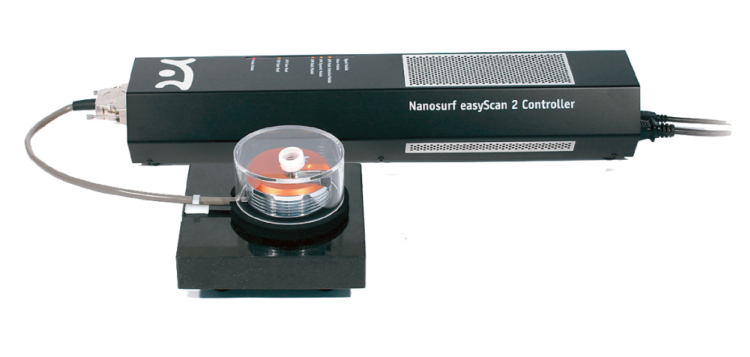
\includegraphics[width=14cm]{pics/stm1}
\caption{Photographie des verwendeten RTMs \textit{easyScan 2
STM Version 1.6} (entnommen aus Webseite des Herstellers)} 
 \label{fig:stm1}
\end{figure}

